\documentclass [a4paper, 11pt] {article}

%document configuration
\newcommand{\courseName}{Machine Learning in Graphics \& Vision}
\newcommand{\termYear}{Summer Term 2020}
\newcommand{\homeworkNum}{3}
\newcommand{\studentOne}{Driton Goxhufi}
\newcommand{\studentTwo} {Damir Ravlija}
\newcommand{\matrikelNrStOne}{4233242}
\newcommand{\matrikelNrStTwo}{5503184}
\newcommand{\mailStOne}{driton.goxhufi@student.uni-tuebingen.de}
\newcommand{\mailStTwo}{damir.ravlija@student.uni-tuebingen.de}

%packages
\usepackage [english] {babel}
\usepackage [T1] {fontenc}
\usepackage [utf8] {inputenc}
\usepackage {graphicx}
\usepackage {subcaption}
\usepackage {amsmath}
\usepackage {amssymb}
\usepackage {amstext}
\usepackage {amsthm}
\usepackage {listings}
\usepackage {tikz}
\usepackage[
pdftex,
pdfauthor={Goxhufi, Driton; Ravlija, Damir},
pdftitle={MLGV - Exercise \homeworkNum Submission},
pdfsubject={Machine Learning in Graphics \& Vision Homework}
]{hyperref}

\usepackage[a4paper,lmargin={2cm},rmargin={2cm},tmargin={3.5cm},bmargin = {2.5cm},headheight = {4cm}]{geometry}

\usepackage[shortlabels]{enumitem}
\usepackage{lastpage}
\usepackage{fancyhdr}

\usepackage{lipsum}
\usepackage{ifthen}

\pagestyle{fancy}



%other config
\renewcommand{\v}[1]{\boldsymbol{#1}}
\newcommand{\mat}[1]{\boldsymbol{#1}}
\newcommand{\m}[1]{\begin{pmatrix}#1\end{pmatrix}}
\newcommand{\tr}[2]{{}^{#1}T_{#2}}
\graphicspath{{./images/}}


\lhead{\begin{tabular}{l}
		\courseName\\
		\termYear \\
		Exercise \homeworkNum
\end{tabular}}
\rhead{\begin{tabular}{lr}
		\studentOne & \matrikelNrStOne \\
		\studentTwo & \matrikelNrStTwo \\
\end{tabular}}

\begin{document}
	
\title{\vspace{-1.5cm}\textbf{Exercise \homeworkNum} \\ 
	\courseName}
\author{\begin{tabular}{lcr}
		\studentOne & \matrikelNrStOne & \href{mailto:\mailStOne}{\mailStOne} \\
		\studentTwo & \matrikelNrStTwo & \href{mailto:\mailStTwo}{\mailStTwo} 
\end{tabular}}	
\date{}
\maketitle


\section*{Task 1}
\begin{enumerate}
\item[(a)]
Our implementation does achieve 97.05\% accuracy after 15 epochs.\\
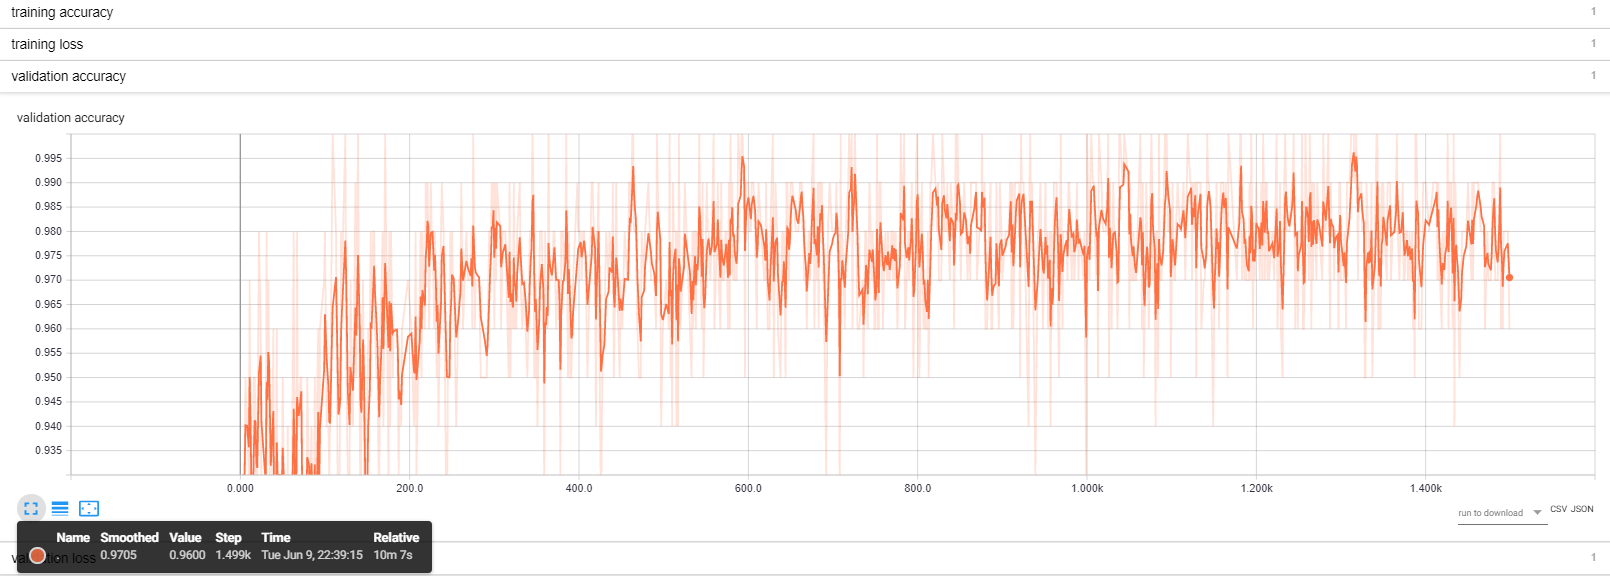
\includegraphics{img/validation_acc_15epochs.png}\\
According to \url{http://rodrigob.github.io/are_we_there_yet/build/classification_datasets_results.html#4d4e495354} the paper "Regularization of Neural Networks using DropConnect" in 2013 achieved a result of 0.21\% errorrate, hence an accuracy value of 99.79\%.

\item[(b)]
from torchsummary import summary\\
summary(model, (1,28,28))\\
----------------------------------------------------------------\\
Layer (type)               Output Shape         Param \#\\
==========================\\
Conv2d-1           [-1, 32, 28, 28]             320\\
ReLU-2           [-1, 32, 28, 28]               0\\
Conv2d-3           [-1, 32, 28, 28]           9,248\\
ReLU-4           [-1, 32, 28, 28]               0\\
Conv2d-5           [-1, 32, 28, 28]           9,248\\
Linear-6                  [-1, 256]       6,422,784\\
ReLU-7                  [-1, 256]               0\\
Linear-8                   [-1, 10]           2,570\\
==========================\\
Total params: 6,444,170\\
Trainable params: 6,444,170\\
Non-trainable params: 0\\
----------------------------------------------------------------\\
Input size (MB): 0.00\\
Forward/backward pass size (MB): 0.96\\
Params size (MB): 24.58\\
Estimated Total Size (MB): 25.55\\
----------------------------------------------------------------\\

Output of convolutional layers can be calculated with this formula: 

\begin{align*}
\left[(W-K+2P)/S\right]+1 \\
\end{align*}

where $W$ is the width(or height if the input is squared), $K$ is the kernelsize, $P$ is the amount of padding and $S$ the stride.

\item[(c)]
After 15 epochs training on the default network with FashionMNIST dataset, \\
the validation(test) accuracy is about 89\%.\\
Console output:\\
epoch done:  14
accuracy train 0.9082844034830729
accuracy test 0.891600112915039\\
\\

We then increased the size of the network in a fashion similar to VGG network. We used stride 2 to speed up training and decrease the number of features while simultaneously incresing the number of filters. To increase the training speed we added batch normalization layers. The following network had the highest accuracy of $0.9108000755310058$ on the validation set (the corresponding accuracy curves are in Figure \ref{fig:2}):

\begin{lstlisting}
----------------------------------------------------------------
Layer (type)               Output Shape         Param #
================================================================
Conv2d-1           [-1, 32, 28, 28]             320
BatchNorm2d-2           [-1, 32, 28, 28]              64
ReLU-3           [-1, 32, 28, 28]               0
Conv2d-4           [-1, 32, 14, 14]           9,248
BatchNorm2d-5           [-1, 32, 14, 14]              64
ReLU-6           [-1, 32, 14, 14]               0
Conv2d-7           [-1, 32, 14, 14]           9,248
BatchNorm2d-8           [-1, 32, 14, 14]              64
ReLU-9           [-1, 32, 14, 14]               0
Conv2d-10             [-1, 64, 7, 7]          18,496
BatchNorm2d-11             [-1, 64, 7, 7]             128
ReLU-12             [-1, 64, 7, 7]               0
Conv2d-13             [-1, 64, 7, 7]          36,928
BatchNorm2d-14             [-1, 64, 7, 7]             128
ReLU-15             [-1, 64, 7, 7]               0
Conv2d-16             [-1, 64, 7, 7]          36,928
BatchNorm2d-17             [-1, 64, 7, 7]             128
ReLU-18             [-1, 64, 7, 7]               0
Conv2d-19            [-1, 128, 4, 4]          73,856
BatchNorm2d-20            [-1, 128, 4, 4]             256
ReLU-21            [-1, 128, 4, 4]               0
Conv2d-22            [-1, 128, 4, 4]         147,584
BatchNorm2d-23            [-1, 128, 4, 4]             256
ReLU-24            [-1, 128, 4, 4]               0
Conv2d-25            [-1, 128, 4, 4]         147,584
BatchNorm2d-26            [-1, 128, 4, 4]             256
ReLU-27            [-1, 128, 4, 4]               0
Conv2d-28            [-1, 256, 2, 2]         295,168
BatchNorm2d-29            [-1, 256, 2, 2]             512
ReLU-30            [-1, 256, 2, 2]               0
Conv2d-31            [-1, 512, 2, 2]       1,180,160
BatchNorm2d-32            [-1, 512, 2, 2]           1,024
ReLU-33            [-1, 512, 2, 2]               0
Conv2d-34            [-1, 512, 2, 2]       2,359,808
BatchNorm2d-35            [-1, 512, 2, 2]           1,024
ReLU-36            [-1, 512, 2, 2]               0
Conv2d-37            [-1, 512, 2, 2]       2,359,808
BatchNorm2d-38            [-1, 512, 2, 2]           1,024
ReLU-39            [-1, 512, 2, 2]               0
Conv2d-40           [-1, 1024, 1, 1]       4,719,616
BatchNorm2d-41           [-1, 1024, 1, 1]           2,048
ReLU-42           [-1, 1024, 1, 1]               0
Conv2d-43           [-1, 1024, 1, 1]       9,438,208
BatchNorm2d-44           [-1, 1024, 1, 1]           2,048
ReLU-45           [-1, 1024, 1, 1]               0
Conv2d-46           [-1, 1024, 1, 1]       9,438,208
BatchNorm2d-47           [-1, 1024, 1, 1]           2,048
ReLU-48           [-1, 1024, 1, 1]               0
Linear-49                   [-1, 10]          10,250
================================================================
Total params: 30,292,490
Trainable params: 30,292,490
Non-trainable params: 0
----------------------------------------------------------------
Input size (MB): 0.00
Forward/backward pass size (MB): 1.45
Params size (MB): 115.56
Estimated Total Size (MB): 117.01
----------------------------------------------------------------
\end{lstlisting}


\begin{figure}[!h]
	\centering
	\begin{subfigure}{0.7\textwidth}
		\centering
		\includegraphics[width=\textwidth]{3-1-c-train.png}
		\caption{Training accuracy curve}
		\label{fig:2a}
	\end{subfigure}
	\begin{subfigure}{0.7\textwidth}
		\centering
		\includegraphics[width=\textwidth]{3-1-c-valid.png}
		\caption{Validation accuracy curve}
		\label{fig:2b}
	\end{subfigure}
	\caption{Plot of results from task 3.1.c)}
	\label{fig:2}
\end{figure}

As we can see from the plots (Figure \ref{fig:2}) it seems that our network overfits the data and it could benefit from early stopping.


% TODO:
\item[(d)]

\end{enumerate}

\section*{Task 2}
\begin{enumerate}
	\item[(a)] Visualization of the image pairs. Every noisy image is located in front of the original image (Figure (\ref{fig:2-a})).
	
	\begin{figure}[!h]
		\centering
		\includegraphics[width=0.8\textwidth]{3-2-a.jpg}
		\caption{Sample of image pairs contained in the \texttt{NoisyFashionMNIST}}
		\label{fig:2-a}
	\end{figure}
\end{enumerate}
	
\end{document}

